%% Use the hmcposter class with the thesis document-class option.
\documentclass[thesis]{hmcposter}
\usepackage{graphicx}
\usepackage{natbib}
\usepackage{booktabs}
\usepackage{subfig}
\usepackage{amsmath}
\usepackage{textcomp}
\usepackage{url}

%% Author of the thesis.
\author{Jenny Lee}

%% The year of your thesis poster's creation.
\posteryear{2018}

%% Thesis Title.
\title{On Self-Regulation in\\College-Level Math Classes}

%% The name of the class for which the poster was created.
%% Generally we see posters for thesis and Clinic, but sometimes
%% other classes require or allow the creation of posters to
%% communicate the results of a project.
%%
%% Use the format Math nnn: Class Title.
\class{Math 197: Senior Thesis}

%% Advisor(s) name or names.  Separate with \and.
\advisor{Dagan Karp}

%% Reader(s) name or names.  Separate with \and.
\reader{Luis A. Leyva (Vanderbilt University)}


%% Define the \BibTeX command, used in our example document.
\providecommand{\bibtex}{{\rmfamily B\kern-.05em%
    \textsc{i\kern-.025em b}\kern-.08em%
T\kern-.1667em\lower.7ex\hbox{E}\kern-.125emX}}

\pagestyle{fancy}

\begin{document}

\begin{poster}

\section{Introduction}
% Note that we're not labeling sections because you shouldn't be
% doing a lot of referring back and forth in your poster---let the
% interested folks read your thesis or Clinic report, or ask
% questions.
What does it mean for mathematics to be fair?

Postsecondary mathematics education in the US has largely looked similar throughout the last century, with lecture-based classes, weekly homework assignments, and two or three exams. Teaching methods have not changed much, and this presents a problem of inequity where some students benefit while others are biased against. Furthermore, mathematics classrooms tend be led by one instructor lecturing a class of ten to upwards of hundreds of students. This dynamic raises questions of where the locus of power is today and whether this should be shifted more to students.

This thesis tries to look into incorporating self-regulation into a mathematics classroom at the college-level. A case study using self-paced assessments was conducted to potentially pose a question on whether self-regulation is a way to reduce inequity in the classroom.


\section{Status Quo}
The lecture-based style of mathematics classrooms today is beneficial only to some. A look into how this happens can be categorized in, but not limited to, largely three different levels.

\begin{itemize}
  \item Implicit Biases by Instructors
  \item Structural Biases in Institutions
  \item Cultural Obstructions
\end{itemize}

Each of these are explained through the analysis of works done by various educators and psychologists, starting from results of the Harvard implicit bias study to socioeconomic differences to historical dehumanization of students. Why certain inequities exist in mathematics education at postsecondary levels, and why they continue to exist, shine light into why mathematics education reform is needed.

\section{Self-regulation}

Self-regulation is not a specified method of learning but rather a skill that students can learn. The purpose of self-regulation is to foster self-generated thought and actions, cyclically adapted to fit personal goals and needs \citep{boekaerts}.

This definition sheds light into how students can have more agency over their own learning, which may shift the locus of power from being purely centralized to the instructor.

\section{For Further Information}
Please contact me through the following ways for further questions or comments:
\begin{itemize}
\item Email: \url{jelee@hmc.edu}
\item Website: \url{https://sites.google.com/g.hmc.edu/jlee/home}
\item Thesis: \url{https://sites.google.com/g.hmc.edu/jlee/thesis}
\item Poster: \url{https://sites.google.com/g.hmc.edu/jlee/poster}
\end{itemize}


\vfill
\columnbreak

\section{Method}%

\begin{figure}
\begin{center}
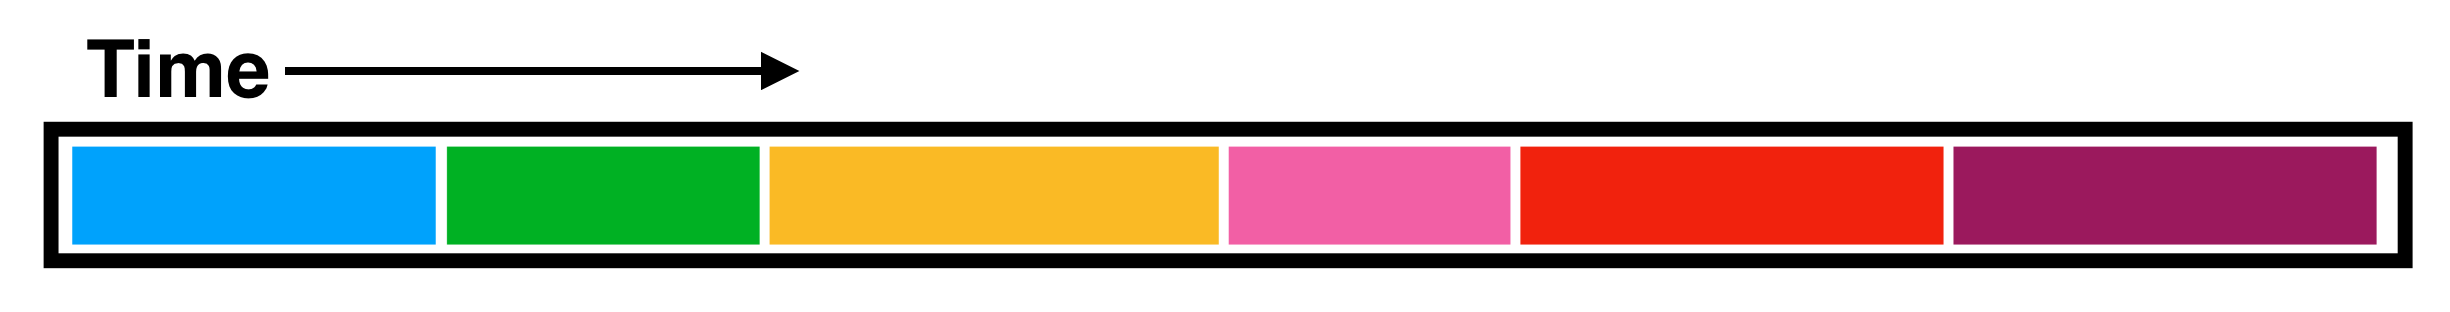
\includegraphics[width=12in]{units}
\caption{An simple example of topics covered over a semester. Each of the six colored segments represents one possible time frame a topic is covered.}%
\end{center}
\end{figure}

\begin{figure}
\begin{center}

\includegraphics[width=12in]{trad}
\caption{One midterm and final exams shown in two blocks with possible proportions of material covered.}%
\end{center}
\end{figure}

\begin{figure}
\begin{center}
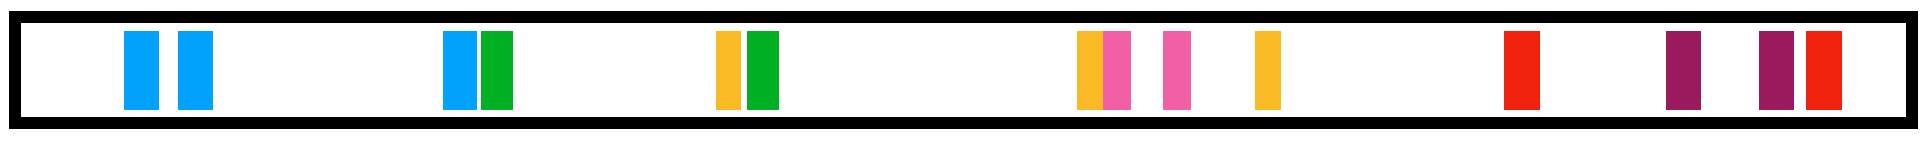
\includegraphics[width=12in]{spa}
\caption{One possible way a student could have taken self-paced assessments throughout the semester, shown as multiple small blocks, each building over the course of the semester.}%
\end{center}
\end{figure}

The case study was conducted at Harvey Mudd College, with 49 first-year students in the introductory linear algebra course (Math 40). There were two sections under study, one of which would be the control. The control section students received weekly assignments, one midterm and one final exam. The test section students received the same weekly assignments but received 10 self-paced assessments, which would be completed and turned in during their own time throughout the semester. These self-paced assessments could be retaken at any time without supervision, and the final grade of each would be determined by their best attempt. Since the only deadline was the end of the semester, students were expected to be mindful of their own test scheduling.

\section{Results}%
The case study was done with a group of 49 students. Results showed no significant differences in academic achievement, but qualitative comments from students showed this method reduced stress and increased self-regulation in the test section. For instance, students commented that they needed to be aware of making sure assessments wouldn't pile up (an example of self-regulation) and others commented they helped review material from earlier in the semester. Overall, the study showed possibilities that self-paced assessments may be something to consider in other courses and different institutions.

\bibliographystyle{hmcmath}
\bibliography{sampleposter}

\vfill

\section{Acknowledgments}
I want to express my appreciation to Professor Karp and the Department of Mathematics at Harvey Mudd College for supporting my research and fostering my interests in mathematics education. I also am thankful for Professor Luis A. Leyva at Vanderbilt University for graciously reading and providing feedback, as well as for advocating and pursuing equitable educational measures in his work.

\vfill
\end{poster}

\end{document}
